\documentclass[12pt, a4paper, simple]{eskdtext}

\usepackage{_env/gpi_global.env}
\usepackage{_env/gpi_report.env}
\usepackage{_sty/gpi_lst}
\usepackage{_sty/gpi_toc}
\usepackage{_sty/gpi_t}
\usepackage{_sty/gpi_u}

\def \gpiDocTopic {Отчёт лабораторной работы №\gpiDocNum}

\begin{document}
\begin{ESKDtitlePage}
    \ESKDstyle{empty}
    \begin{center}
        \gpiMinEduRep \\
        \gpiEduRep \\
        \gpiKafRep \\
    \end{center}

    \vfill

    \begin{center}
        Тема: <<\gpiTopicRep>>
    \end{center}

    \vfill

    \begin{center}
        \textbf{\gpiDocTopic} \\
        по дисциплине \gpiDisciplineRep \\
    \end{center}

    \vfill

    \begin{flushright}
        \begin{minipage}[t]{7cm}
            Выполнил: \\
            \PageTitleStudentInfo \\
            \hspace{0pt} \\
            Проверил: \\
            \PageTitleTeacherInfo \\
        \end{minipage}
    \end{flushright}

    \vfill

    \begin{center}
        \PageTitleCity~\ESKDtheYear
    \end{center}
\end{ESKDtitlePage}


\ESKDstyle{empty}

\begin{center}
    \textbf{\gpiDocTopic}
\end{center}

\paragraph{} \textbf{Тема}: <<\gpiTopicRep>>

\paragraph{} \textbf{Цель}:
\begin{enumerate}
    \item[1.] Необходимо разработать алгоритм решения задачи (в соответствии c вариантом)
    \item[2.] Разработать словесное описание алгоритма решения задачи
    \item[3.] Разработать блок - схему решения поставленной задачи.
    \item[4.] Блок - схему реализовать в соответствии c ГОСТ
    \item[5.] Блок - схему алгоритма начертить в Visio (или open-source draw.io)
\end{enumerate}

\paragraph{} \textbf{Что нужно сделать}:

\begin{center}
    \textbf{Вариант 5}
\end{center}

Задан круг с центром в точке $O(x_0, y_0)$ и радиусом $R_0$ и точка $A(x_1, y_1)$.
Определить месторасположение точки по отношению к кругу
(находится внутри круга, вне его или лежит на окружности).

\paragraph{} \textbf{Словесное описание алгоритма}:

\begin{enumerate}
    \item[1.] Получаем параметры $x_0, y_0, R_0, x_1, y_1$. Переход к указанию 2.
    \item[2.] Вычисляем $R1 = \sqrt{(x_1 - x_0)^2 + (y_1 - y_0)^2}$. Переход к указанию 3.
    \item[3.] Если $R_1 > R_0$, то переход к указанию 3.1, иначе переход к указанию 4.
    \item[3.1] Выводим сообщение: "Точка за окружностью". Переход к указанию 3.2.
    \item[3.2] Выход из функции. Переход к указанию 7.
    \item[4] Если $R_1 < R_0$, то переход к указанию 4.1, иначе переход к указанию 5.
    \item[4.1] Выводим сообщение: "Точка в окружности". Переход к указанию 4.2.
    \item[4.2] Выход из функции. Переход к указанию 7.
    \item[5] Выводим сообщение: "Точка на окружности". Переход к указанию 6.
    \item[6] Выход из функции. Переход к указанию 7.
    \item[7] Конец.
\end{enumerate}

\paragraph{} \textbf{Блок-схема алгоритма}:

Блок-схема алгоритма изображена на рисунке~\ref{fig:5}.

\begin{figure}[!ph]
    \centering
    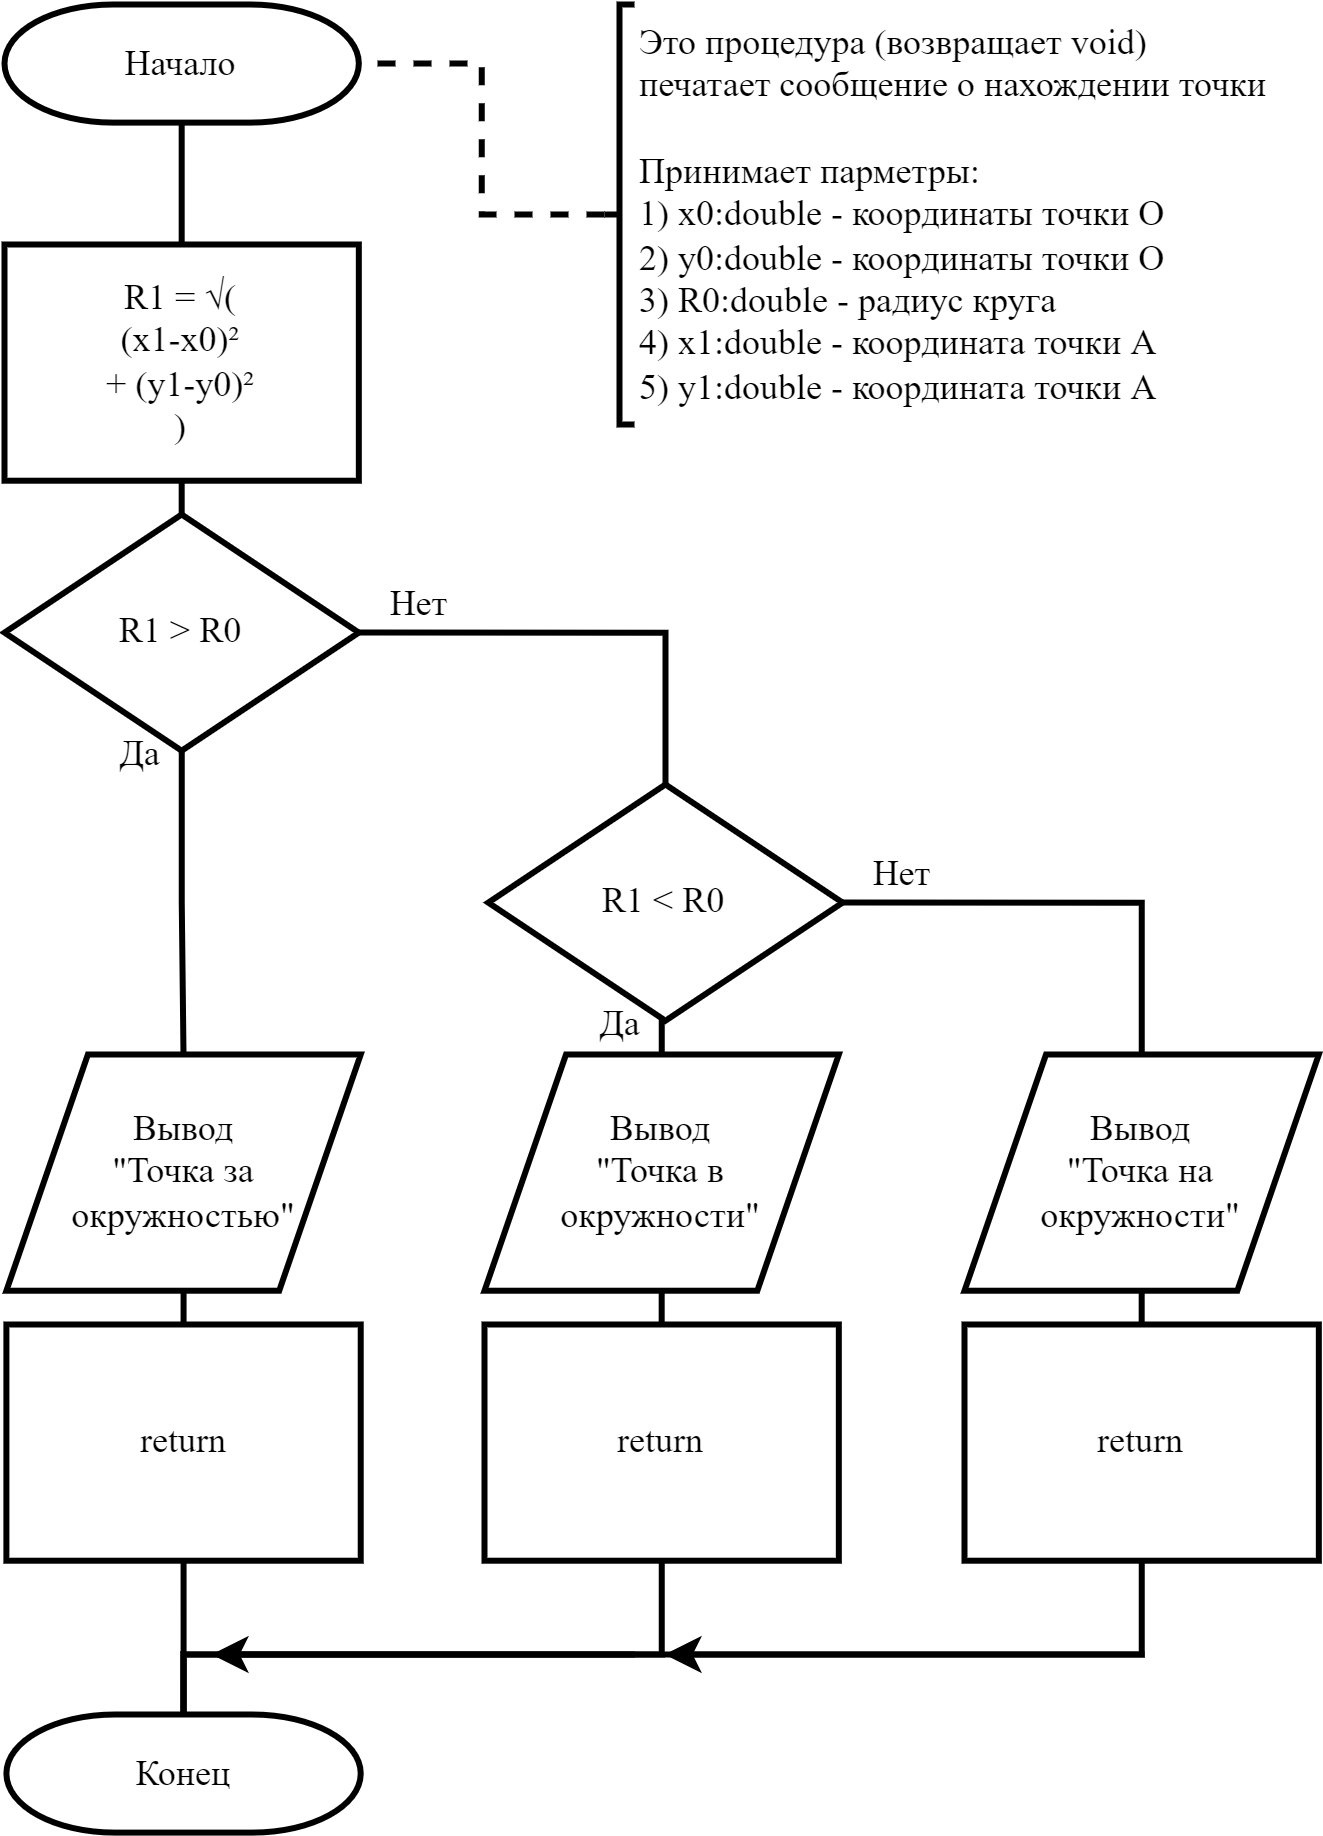
\includegraphics[]
    {../sources/flowcharts/5.png}
    \caption{Дизайн}
    \label{fig:5}
\end{figure}

\paragraph{} \textbf{Вывод}:
Разработал алгоритм для своей задачи.
Разработал словесное описание алгоритма.
Разработал блок-схему решения задачи.
Реализовал блок-схему в соотвествии с ГОСТ.
Нарисовал блок-схему в open-source draw.io.

% = = = = = = = =
\newpage
% \addcontentsline{toc}{section}{Список использованных источников}
% \section*{Список использованных источников}
\paragraph{} \textbf{Список использованных источников}:
\begin{enumerate}
    \item[1.] Коллекция eskdx v0.98 - eskdx.pdf
    [Электронный ресурс].
    Режим доступа: \url{http://tug.ctan.org/macros/latex/contrib/eskdx/manual/eskdx.pdf}.
    Дата доступа: 30.05.2022.

    \item[2.] Использование системы верстки LaTeX - EVMiS\_Latex.pdf
    [Электронный ресурс].
    Режим доступа: \url{https://www.bstu.by/uploads/attachments/metodichki/kafedri/EVMiS_Latex.pdf}.
    Дата доступа: 30.05.2022.

    \item[3.] Опции пакета hyperref
    [Электронный ресурс].
    Режим доступа: \url{https://grammarware.net/text/syutkin/hyperref_options.pdf}.
    Дата~доступа:~20.02.2022.

    \item[4.] Developers - Docker
    [Electronic resource].
    Mode of access: \url{https://www.docker.com/get-started/}.
    Date~of~access:~04.06.2022.

    \item[5.] Manual installation steps for older versions of WSL | Microsoft Docs
    [Electronic resource].
    Mode of access: \url{https://aka.ms/wsl2kernel}.
    Date~of~access:~04.06.2022.

    \item[6.] LaTeX/Source Code Listings - Wikibooks, open books for an open world
    [Electronic resource].
    Mode of access: \url{https://en.wikibooks.org/wiki/LaTeX/Source_Code_Listings}.
    Date~of~access:~04.06.2022.

    \item[7.] 1sem\_OAiP/OAiP\_lab2.doc at galanin · BrSTU-PO4-Galanin/1sem\_OAiP
    [Электронный ресурс].
    Режим доступа: \url{https://github.com/BrSTU-PO4-Galanin/1sem_OAiP/blob/galanin/docs/lab2/OAiP_lab2.doc}.
    Дата~доступа:~05.06.2022.
\end{enumerate}

\newpage
\end{document}
